\chapter{Cardinality Estimation Model (Experimental Evaluation)}
\chaptermark{Evaluation}

\begin{aboutchapter}
In Chapter \ref{chap:neo4j-impl} we have defined estimations for the
cardinalities of query results in a graph database and explained how they
can be implemented in Neo4j.
In this Chapter, we evaluate our implementation using a benchmark and
compare it with Neo4j's current implementation.
\end{aboutchapter}

\section{Test setting}

We compare our cardinality estimations with the estimations of Neo4j version
"3.1.0-M08" (Maven version)%
\footnote{\url{https://mvnrepository.com/artifact/org.neo4j/neo4j/3.1.0-M08}}.

Our test takes a database and a catalog of queries on this database as input.
It outputs a CSV-file containing the actual result cardinality of the query and
the estimated cardinality of our and Neo4j's estimation model:
\begin{figure}[H]
  \centering
  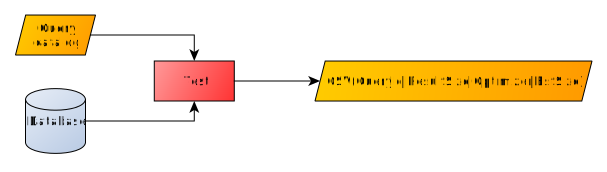
\includegraphics[width=0.9\textwidth]{figures/testbed.pdf}
  \caption{The test setting.}
  \label{fig:testbed}
\end{figure}

The platform of execution is not relevant, because the measured variables
(result size and estimated sizes) are platform-independent.

\subsection{Query Dimensions}
\label{sec:query-dimensions}

As discussed in Section \ref{sec:cypher-to-operators}, our cardinality
estimations cover all CSP queries that map to a tree subgraph pattern.
% For this query space, our test compares our estimations with the
% estimations of Neo4j.
Within this query space, we can group queries according to several
important dimensions:
\begin{samepage}
\begin{enumerate}
  \renewcommand{\labelenumii}{\theenumii}
  \renewcommand{\theenumii}{\theenumi.\arabic{enumii}.}
  \renewcommand{\theenumiii}{\theenumii\arabic{enumiii}}
  
  \item Query shapes
    \begin{enumerate}
      \item Chain queries (denoted by --)
      \item Star queries (denoted by *)
      \item Snowflake queries (denoted by \#)
    \end{enumerate}
  \item Type constraints
    \begin{enumerate}
      \item Queries without type constraints
      \item Queries with type constraints
    \end{enumerate}
  \item Label constraints
    \begin{enumerate}
      \item Queries without label constraints
      \item Queries with label constraints
      \begin{enumerate}
        \item Queries with redundant label constraints (explanation below)
        \item Queries where labels are in a sublabel relation
        \item Queries where labels are disjoint
        \item Queries where labels are (approximately) independent
      \end{enumerate}
    \end{enumerate}
\end{enumerate}
\end{samepage}

We call a label constraint on a node variable \emph{redundant}, if the label is
already determined by the type of a relationship connected to the node
variable.
E.g. in the SNB schema shown below, if a node variable is connected to an
outgoing relationship of type "HAS\_INTEREST", adding "Person" as a label
constraint on this node variable is redundant.

In order to be representative, a catalog of test queries should cover most of
the value combinations of the given dimensions.

\subsection{Dataset: The LDBC Social Network Benchmark}

According to the homepage:
\begin{quote}
"The Social Network Benchmark (SNB) consists of a data generator that generates
a synthetic social network, used in three workloads: Interactive, Business
Intelligence and Graph Analytics. Currently, only the Interactive Workload has
been released in draft stage."

(\url{http://ldbcouncil.org/developer/snb}, 06/04/2017)
\end{quote}

We use the dataset of the Interactive workload
\cite{erling_ldbc_2015} with default settings.

\subsubsection{Importing the Dataset}

After executing the data generator%
\footnote{\url{https://github.com/ldbc/ldbc_snb_datagen}, 1.6.2017}, the
generated CSV files have to be imported into Neo4j using the Neo4j import
tool%
\footnote{\url{https://neo4j.com/docs/operations-manual/3.1/tools/import/},
5.6.2017}.
The import requires a reformatting of the CSV files, which can be achieved by
Jonathan Ellithorpe's \emph{DataFormatConverter}%
\footnote{\url{https://github.com/PlatformLab/ldbc-snb-impls/blob/%
6d52ca5cc492ca8aeffed4cbbdcf7d1a6c073061/snb-interactive-neo4j/%
src/main/java/net/ellitron/ldbcsnbimpls/interactive/neo4j/util/%
DataFormatConverter.java}, 5.6.2017}.
% However, the mapping used in the DataFormatConverter uses a property "type" to
% differentiate between the subclasses of the Place and Organisation classes.
% Because we do not consider properties in our graph model, we add the
% respective labels (City, Country, Continent, University, Company) to the
% subclasses after the import.

\subsubsection{Label Partition and Sublabel Map}

The schema of the SNB data is shown in Figure \ref{fig:snb-schema}.
The mapping to a property graph performed by the \texttt{DataFormatConverter}
uses a property "type" to differentiate between the subclasses of the Place and
Organisation classes.
Because we do not consider properties in our graph model, we add the
respective labels (City, Country, Continent, University, Company) to the
subclasses after the import.
After this step, all classes in the schema map directly to node labels in
our database.

\begin{figure}
  \centering
  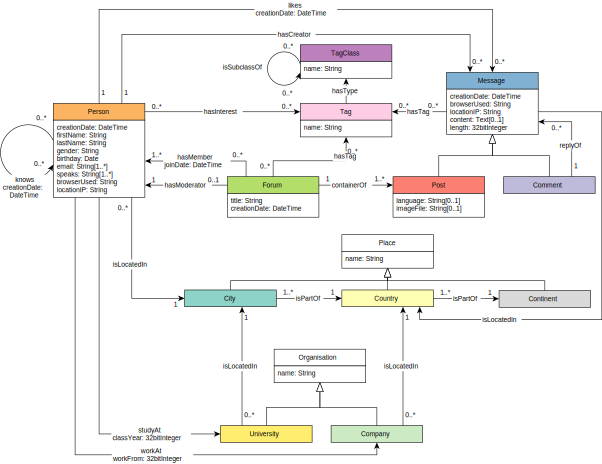
\includegraphics[width=\textwidth]{figures/snb_schema.pdf}
  \caption{Schema of the SNB Interactive workload. Taken from
  \textit{LDBC SNB Documentation 0.3.0},
  \url{https://github.com/ldbc/ldbc_snb_docs},
  06/04/2017.}
  \label{fig:snb-schema}
\end{figure}

Observe that every node in the database has at least one label.
Furthermore, any two different labels in the SNB schema are either disjoint or
in a sublabel relation.
This label distribution can be stored in a label partition and a sublabel
map, which are needed by our estimations.
We use the strict label partition and the strict sublabel map
(cf. Section \ref{sub:sublabel-map}).
The strict label partition is given as
\begin{align}
\begin{split}
  \lpart_\snb := \{ &\{ \text{Message}, \text{Post}, \text{Comment} \}, \\
                    &\{ \text{Place}, \text{Continent}, \text{Country},
                        \text{City} \}, \\
                    &\{ \text{Organisation}, \text{University},
                        \text{Company} \}, \\
                    &\{ \text{Person} \}, \\
                    &\{ \text{Forum} \}, \\
                    &\{ \text{Tag} \}, \\
                    &\{ \text{TagClass} \} \}
\end{split}
\end{align}

The strict sublabel map is given as
\begin{align}
\begin{split}
  &\submap_\snb(\text{Message}) := \{ \text{Post}, \text{Comment} \}, \\
  &\submap_\snb(\text{Post}) := \emptyset \\
  &\submap_\snb(\text{Comment}) := \emptyset \\
  &\submap_\snb(\text{Place}) := \{ \text{Continent}, \text{Country},
                                    \text{City} \}, \\
  &\submap_\snb(\text{Continent}) := \emptyset \\
  &\submap_\snb(\text{Country}) := \emptyset \\
  &\submap_\snb(\text{City}) := \emptyset \\
  &\submap_\snb(\text{Organisation}) := \{ \text{University},
                                           \text{Company} \}, \\
  &\submap_\snb(\text{University}) := \emptyset \\
  &\submap_\snb(\text{Company}) := \emptyset \\
  &\submap_\snb(\text{Person}) := \emptyset \\
  &\submap_\snb(\text{Forum}) := \emptyset \\
  &\submap_\snb(\text{Tag}) := \emptyset \\
  &\submap_\snb(\text{TagClass}) := \emptyset
\end{split}
\end{align}

\subsection{Query Catalog}

The queries contained in the  SNB Interactive workload exceed by far what we
can express in our current query algebra.
Therefore, we select a subset of interesting queries in the SNB schema and
compare the cardinality estimations of our model and Neo4j's model on this
subset.

Tables \ref{table:query-catalog-1}, \ref{table:query-catalog-2} and
\ref{table:query-catalog-3}  show our query catalog for the SNB.
For each query, the table lists the unique query id, the Cypher pattern,
the query shape and whether the query has type or label constraints.

Our query catalog covers most of the value combinations of the query dimensions
specified in Section \ref{sec:query-dimensions}.
However, due to the SNB schema, it does not occur that two labels are
(approximately) independent.

\begin{landscape}
  \begin{table}[h]
    \includegraphics[width=\linewidth]{tables/snb-query-catalog/query_catalog_1.pdf}
    \caption{The catalog of test queries for the SNB (part 1).}
    \label{table:query-catalog-1}
  \end{table}
  \begin{table}[h]
    \includegraphics[width=\linewidth]{tables/snb-query-catalog/query_catalog_2.pdf}
    \caption{The catalog of test queries for the SNB (part 2).}
    \label{table:query-catalog-2}
  \end{table}
  \begin{table}[h]
    \includegraphics[width=\linewidth]{tables/snb-query-catalog/query_catalog_3.pdf}
    \caption{The catalog of test queries for the SNB (part 3).}
    \label{table:query-catalog-3}
  \end{table}
\end{landscape}

\section{Analysis}

The complete results of our tests can be found in Appendix
\ref{app:test-results}.

\subsection{Comparison of the Correlation between Actual and Estimated
            Result Cardinalities}

For any predictive model it is desirable that its predictions are strongly
linearly correlated with the actual observations.
A strong linear correlation means that, the model behaves like reality
(apart from a constant shift and rescaling).

For our cardinality estimations, a strong linear correlation
between the actual result cardinality and the estimated cardinality
implies for instance that, if query A has a smaller result cardinality than
query B, the estimated cardinality of A will probably also be smaller than
the estimated cardinality of B.
This property is crucial for any optimizer, in order to choose the execution
plan where the intermediate cardinalities are minimal.

Our hypothesis is that, our estimations are \emph{significantly}
more correlated with the actual result cardinalities than Neo4j's estimations,

In order to prove this hypothesis, we have to use statistical tests.
We compute these tests in R, using the \emph{cocor} package%
\cite{diedenhofen_cocor:_2015}%
\footnote{\url{https://cran.r-project.org/web/packages/cocor/index.html},
18.06.2017}.
Cocor computes several tests at once, including Pearson and Filon's z-test.

In the following R code, the variables have the following meaning:
\begin{itemize}
  \item \texttt{ResultSize} is the actual result cardinality of a query.
  \item \texttt{Neo4jEstSize} is Neo4j's estimate of the result cardinality
    of a query.
  \item \texttt{CascadesEstSize} is our estimate of the result cardinality
    of a query.
\end{itemize}

We want to show that our estimations correlate better with the actual result
cardinalities than the estimations of Neo4j.

The corresponding null hypothesis is that, the correlation between
\texttt{ResultSize} and \texttt{Neo4jEstSize} is greater or equal than
the correlation between
\texttt{ResultSize} and \texttt{CascadesEstSize}.

The following R statement runs the test:
\begin{verbatim}
cocor(~ResultSize + EstNeo4j | ResultSize + EstCascades,
      t, alternative = "less", conf.level = 0.99)
\end{verbatim}

The test output tells us, that the actual result cardinality
is only marginally correlated with the estimations of Neo4j ($r = 0.0409$),
but strongly correlated with our estimations ($r = 0.8258$).

Moreover, Table \ref{table:cocor-test-results} shows that all tests run by
cocor tell us to reject our null hypothesis at 99\% confidence level
($\alpha = 0.01$)%

\begin{table}
\centering
\caption{Formatted output of the tests run by cocor.}
\label{table:cocor-test-results}
\begin{tabular}{@{}lll@{}}
\toprule
Test name                                                                                                                                                                             & Test result                                                                                           & \begin{tabular}[c]{@{}l@{}}Null\\ hypothesis\\ rejected?\end{tabular} \\ \midrule
Pearson and Filon's z (1898)                                                                                                                                                          & \begin{tabular}[c]{@{}l@{}}z = -4.8927\\ p-value = 0.0000\end{tabular}                                & Yes                                                                   \\
Hotelling's t (1940)                                                                                                                                                                  & \begin{tabular}[c]{@{}l@{}}t = -6.2367\\ df = 41\\ p-value = 0.0000\end{tabular}                      & Yes                                                                   \\
Williams' t (1959)                                                                                                                                                                    & \begin{tabular}[c]{@{}l@{}}t = -5.4285\\ df = 41\\ p-value = 0.0000\end{tabular}                      & Yes                                                                   \\
Olkin's z (1967)                                                                                                                                                                      & \begin{tabular}[c]{@{}l@{}}z = -4.8927\\ p-value = 0.0000\end{tabular}                                & Yes                                                                   \\
Dunn and Clark's z (1969)                                                                                                                                                             & \begin{tabular}[c]{@{}l@{}}z = -4.9999\\ p-value = 0.0000\end{tabular}                                & Yes                                                                   \\
\begin{tabular}[c]{@{}l@{}}Hendrickson, Stanley, and Hills' (1970)\\ modification of Williams' t (1959)\end{tabular}                                                                  & \begin{tabular}[c]{@{}l@{}}t = -6.2169\\ df = 41\\ p-value = 0.0000\end{tabular}                      & Yes                                                                   \\
\begin{tabular}[c]{@{}l@{}}Steiger's (1980) modification of Dunn\\ and Clark's z (1969) using average correlations\end{tabular}                                                       & \begin{tabular}[c]{@{}l@{}}z = -4.8416\\ p-value = 0.0000\end{tabular}                                & Yes                                                                   \\
Meng, Rosenthal, and Rubin's z (1992)                                                                                                                                                 & \begin{tabular}[c]{@{}l@{}}z = -4.7835\\ p-value = 0.0000\end{tabular}                                & Yes                                                                   \\
\begin{tabular}[c]{@{}l@{}}Hittner, May, and Silver's (2003) modification of\\ Dunn and Clark's z (1969) using a\\ backtransformed average Fisher's (1921)\\ Z procedure\end{tabular} & \begin{tabular}[c]{@{}l@{}}z = -4.7825\\ p-value = 0.0000\end{tabular}                                & Yes                                                                   \\
Zou's (2007) confidence interval                                                                                                                                                      & \begin{tabular}[c]{@{}l@{}}99\% confidence\\ interval for r.jk - r.jh:\\ -1.1878 -0.3610\end{tabular} & Yes                                                                   \\ \bottomrule
\end{tabular}
\end{table}


We can therefore conclude that our estimations are
significantly stronger correlated with the actual result size than Neo4j's
estimations.

The complete test output can be found in Appendix \ref{app:cocor-r-snippet}.

\subsection{Comparison of the Estimation Errors}
\label{sec:estimations-errors}

The predictions produced by a model should not only have a strong linear
correlation with real observations, they should also be \emph{close} to the
observations with respect to some error metric.
For our model, we use the \emph{absolute estimation error} and the
\emph{relative estimation error} as error metrics.

\begin{definition}[Absolute and relative estimation error]
Take a CSP query $c$ with result cardinality $x$.
Suppose an optimizer estimates the result cardinality of $c$ as $\hat{x}$.
The absolute error of this estimation is defined as
\[
  \absErr(x, \hat{x}) := | x - \hat{x} |
\]

If $x \not = 0$, the relative error of this estimation is defined as
\[
  \relErr(x, \hat{x}) := \frac{\absErr(x, \hat{x})}{| x |}
\]
\end{definition}

To decide whether there is a significant difference between the estimation
errors of the optimizers, we use the test for paired observations described by
Raj Jain \cite[p.~209]{jain_art_1991}.

For each query of the catalog, we observe the (absolute/relative) estimation
error of both optimizers. For each pair of error observations, we compute the
difference. Then we compute a confidence interval for this difference.
If this confidence interval includes zero, the systems are not significantly
different. If it does not include zero, there is a significant difference
between the (absolute/relative) estimation errors of the optimizers.

% \subsubsection{Comparison With Respect to Query Dimensions}
%
% Using our specified query dimensions, we try to find subsets where the
% (absolute/relative) estimation error of our and Neo4j's estimation model
% differ the most.
%
\subsubsection{Absolute Estimation Error}

Figure \ref{fig:abs-error-snb} shows the absolute estimation error $\epsilon$
of the two estimation models for the queries in the SNB query catalog.
We transform the error scale using the inverse hyperbolic sine%
\footnote{The inverse hyperbolic sine transformation (asinh) allows to cover
many orders of magnitude and is defined for all real numbers.
cf. \url{http://wresch.github.io/2013/03/08/asinh-scales-in-ggplot2.html},
18.06.2017},
because the error values vary by several orders of magnitude.
The figure indicates that our estimations generate the smaller absolute errors.

\begin{figure}
  \centering
  \includegraphics[width=\textwidth]{figures/eval/abs_error_snb.pdf}
  \caption{Absolute errors of our estimations (Cascades, \emph{red})
           and Neo4j's estimations (Neo4j, \emph{blue})
           for the SNB query catalog.}
  \label{fig:abs-error-snb}
\end{figure}

Figure \ref{fig:abs-error-diff-snb} shows the difference $d_\epsilon$
between the absolute
error of Neo4j's estimations and the absolute error of our estimations.
Like above, we transform the scale using the inverse hyperbolic sine.
Again, we see that our estimations generate the smaller absolute
errors for most of the queries in question.

\begin{figure}
  \centering
  \includegraphics[width=\textwidth]{figures/eval/abs_error_diff_snb.pdf}
  \caption{Difference between the absolute error of Neo4j's estimations
           and our estimations for the SNB query catalog.}
  \label{fig:abs-error-diff-snb}
\end{figure}

Table \ref{table:abs-error-diff-stats} shows that
on average, our estimations are $2\,869\,783\,102$ subgraphs closer to the
actual result cardinality than the estimations of Neo4j.

\begin{table}[h]
\centering
\begin{tabular}{@{}lll@{}}
\toprule
n  & $\text{mean}(d_\epsilon)$    & $\text{var}(d_\epsilon)$ \\ \midrule
44 & $2\,869\,783\,102$           & $2.850809 \cdot 10^{20}$ \\ \bottomrule
\end{tabular}
\caption{Sample size, mean and variance of $d_\epsilon$.}
\label{table:abs-error-diff-stats}
\end{table}

In order to test whether the observed difference in absolute errors is already
\emph{significant}, we compute the 99\% confidence interval of $d_\epsilon$
using the simple procedure described by Raj Jain \cite[p.~209]{jain_art_1991}.
Let $t(0.99, n-1)$ denote the $0.99$-quantile of a t-variate with $n-1$
degrees of freedom. Then the confidence interval $c_\epsilon$ is
\begin{align}
\begin{split}
  c_\epsilon &= \text{mean}(d_\epsilon) \pm t(0.99, n - 1)
                 \cdot \sqrt{\frac{\text{var}(d_\epsilon)}{n}} \\
             &= 2869783102 \pm 2.41625
                \cdot \sqrt{\frac{2.850809 \cdot 10^{20}}{44}} \\
             &\approx (-3280563476.14, 9020129680.14)
\end{split}
\end{align}

This confidence interval includes zero. Consequently, our current SNB query catalog
is not sufficient to conclude that our estimations have significantly smaller absolute
estimation errors than Neo4j's estimations.

To be able to prove this in future experiments, we should increase the sample
size (i.e., the number of queries in the catalog) in order to decrease the
variance of $d_\epsilon$ and thus reduce the size of the confidence interval.

\subsubsection{Relative Estimation Error}

The relative estimation error $\eta$ is only defined for queries having a
non-empty result. In our query catalog, these are 31 queries.
Figure \ref{fig:rel-error-snb} shows the relative estimation error
of our and Neo4j's estimation model for these queries.
The figure indicates that our estimations generate the smaller relative errors.

\begin{figure}
  \centering
  \includegraphics[width=\textwidth]{figures/eval/rel_error_snb.pdf}
  \caption{Relative errors of our estimations (Cascades, \emph{red})
           and Neo4j's estimations (Neo4j, \emph{blue})
           for the SNB query catalog.}
  \label{fig:rel-error-snb}
\end{figure}

Figure \ref{fig:rel-error-diff-snb} shows the difference $d_\eta$
between the relative
error of Neo4j's estimations and the relative error of our estimations.
Again, we see that our estimations generate the lower relative
errors for most of the queries.

\begin{figure}
  \centering
  \includegraphics[width=\textwidth]{figures/eval/rel_error_diff_snb.pdf}
  \caption{Difference between the relative error of Neo4j's estimations
           and our estimations for the SNB query catalog.}
  \label{fig:rel-error-diff-snb}
\end{figure}

Table \ref{table:rel-error-diff-stats} shows that
on average, our relative estimation error is $0.8096792$ smaller than
the relative estimation error of Neo4j.

\begin{table}[h]
\centering
\begin{tabular}{@{}lll@{}}
\toprule
n  & $\text{mean}(d_\eta)$ & $\text{var}(d_\eta)$ \\ \midrule
31 & $0.809679$          & $1.661361$             \\ \bottomrule
\end{tabular}
\caption{Sample size, mean and variance of $d_\eta$.}
\label{table:rel-error-diff-stats}
\end{table}

In order to test whether the observed difference in relative errors is already
\emph{significant}, we compute the 99\% confidence interval of $d_\eta$ using
the same procedure as above.
The confidence interval $c_\eta$ is
\begin{align}
\begin{split}
  c_\eta &= \text{mean}(d_\eta) \pm t(0.99, n - 1)
            \cdot \sqrt{\frac{\text{var}(d_\eta)}{n}} \\
         &= 0.809679 \pm 2.452824
            \cdot \sqrt{\frac{1.661361}{31}} \\
         &\approx (0.24185, 1.377507)
\end{split}
\end{align}

This confidence interval is located above zero.
Hence, we can conclude by 99\% significance that our estimations generate
smaller relative errors than Neo4j's estimations.
